
\documentclass[runningheads,a4paper,11pt]{report}

\usepackage{algorithmic}
\usepackage{algorithm}
\usepackage{array}
\usepackage{amsmath}
\usepackage{amsfonts}
\usepackage{amssymb}
\usepackage{amsthm}
\usepackage{caption}
\usepackage{comment}
\usepackage{epsfig}
\usepackage{fancyhdr}
\usepackage{geometry}
\usepackage{graphicx}
\usepackage[colorlinks]{hyperref}
\usepackage[latin1]{inputenc}
\usepackage{multicol}
\usepackage{multirow}
\usepackage{rotating}
\usepackage{setspace}
\usepackage{subfigure}
\usepackage{url}
\usepackage{verbatim}
\usepackage{xcolor}
\usepackage{longtable}
\graphicspath{ {./Images/} }
\geometry{a4paper,top=3cm,left=2cm,right=2cm,bottom=3cm}

\pagestyle{fancy}
\fancyhf{}
\fancyhead[L, R]{Emotion recognition}
\fancyhead[R,L]{Team 3}
\fancyfoot[R,L]{ITSG 2019-2020}
\fancyfoot[L]{\thepage}

\renewcommand{\headrulewidth}{2pt}
\renewcommand{\footrulewidth}{1pt}
\renewcommand{\headrule}{\hbox to\headwidth{%
  \color{lime}\leaders\hrule height \headrulewidth\hfill}}
\renewcommand{\footrule}{\hbox to\headwidth{%
  \color{lime}\leaders\hrule height \footrulewidth\hfill}}

\hypersetup{
pdftitle={artTitle},
pdfauthor={name},
pdfkeywords={pdf, latex, tex, ps2pdf, dvipdfm, pdflatex},
bookmarksnumbered,
pdfstartview={FitH},
urlcolor=cyan,
colorlinks=true,
linkcolor=red,
citecolor=green,
}
% \pagestyle{plain}

\setcounter{secnumdepth}{3}
\setcounter{tocdepth}{3}

\linespread{1}

% \pagestyle{myheadings}

\makeindex


\begin{document}

\begin{titlepage}
\sloppy
\begin{center}
BABE\c S BOLYAI UNIVERSITY, CLUJ NAPOCA, ROM\^ ANIA

FACULTY OF MATHEMATICS AND COMPUTER SCIENCE

\vspace{6cm}

\Huge \textbf{Kids Emotion Recognition}

\vspace{1cm}

\normalsize -- ITSG report --

\end{center}


\vspace{5cm}

\begin{flushright}
\Large{\textbf{Team members}}\\
Tigau-Almasan Alexandra \\
Gorgos Andreea \\
Corman Robert-Marian \\
\end{flushright}

\vspace{4cm}
l
\begin{center}
2019
\end{center}

\end{titlepage}

\pagenumbering{gobble}

\begin{abstract}

    Emotional recognition permits humans to be aware of their social environment, by reading the feelings of other people just by noticing their micro-expressions and tight them to the context situations. Lots of research has already focused on adults' emotion recognition by using artificial intelligence to read non-verbal communication leading to extraordinary results.

    Our project aim is to train an intelligent algorithm (a \textit{Convolutional Neuronal Netowrk}) to distinguish amongst children emotions and to provide the percentage of the emotion that matched best the provided image input.
    The training part of the algorithm has been performed on CAFE \cite{LoBlue2015} data set, which includes photographs from 154 children (90 female models and 64 male models) with ages between 2 and years 8 old.

\end{abstract}

\tableofcontents

\newpage

\listoffigures

\newpage

\setstretch{1.5}

\newpage

\pagenumbering{arabic}

\chapter{Introduction}
\label{chapter:introduction}

\section{What? Why? How?}
\label{section:whatwhyhow}

\subsection{What?}
\label{subsection:what}
\paragraph{}
The problem we want to solve is the kids emotion recognition from images or videos based on 7 emotions: Angry, Disgust, Fear, Happy, Sad, Surprise and Neutral.

\subsection{Why?}
\label{subsection:why}
\paragraph{}
Children are able to recognize certain emotions very well when they are just 6 years old, but become better at recognizing other emotions as they grow older. The data obtained by reading children emotions can be extremely useful when working with children that may suffer from a disorder such as autism \cite{Bal2010} or Down Syndrome  \cite{Kasari2001} or when trying to read emotions from maltreated children who suffered a trauma and integrate them with other emotion cues \cite{Camras1996}. Both the diagnostic and the medical therapy can use emotion recognition to adapt their method to the young patient's needs.

\paragraph{}
Children emotion recognition has applicability in the education domain as well, by developing learning software platforms that could accurately spot the emotion of the children and adapt the learning level to his needs. Another useful learning application would help the children to recognise better the emotions of other people.

\paragraph{}
Subsequently, by identifying children emotions more easily they can be even more targeted by the advertisement industry, tailoring products that respond best to children reactions.
Market researches are nowadays more easily to perform since the participants verbal input may no longer be needed (as long as they are not influenced by any other process thought when expressing an emotion, misleading to a different conclusion of survey).

\paragraph{}
Gaming industry could improve their gaming offer by capturing the children emotions while playing and adapting the level of the game or the scenario according to the player's shown emotions.

\paragraph{}
However, people are still reticent when thinking about allowing a camera to capture their emotions while performing any actions and about the manner in which the collected data will be used afterwards.

\begin{figure}[!ht]
  \label{fig::MindMap}
  \centering
  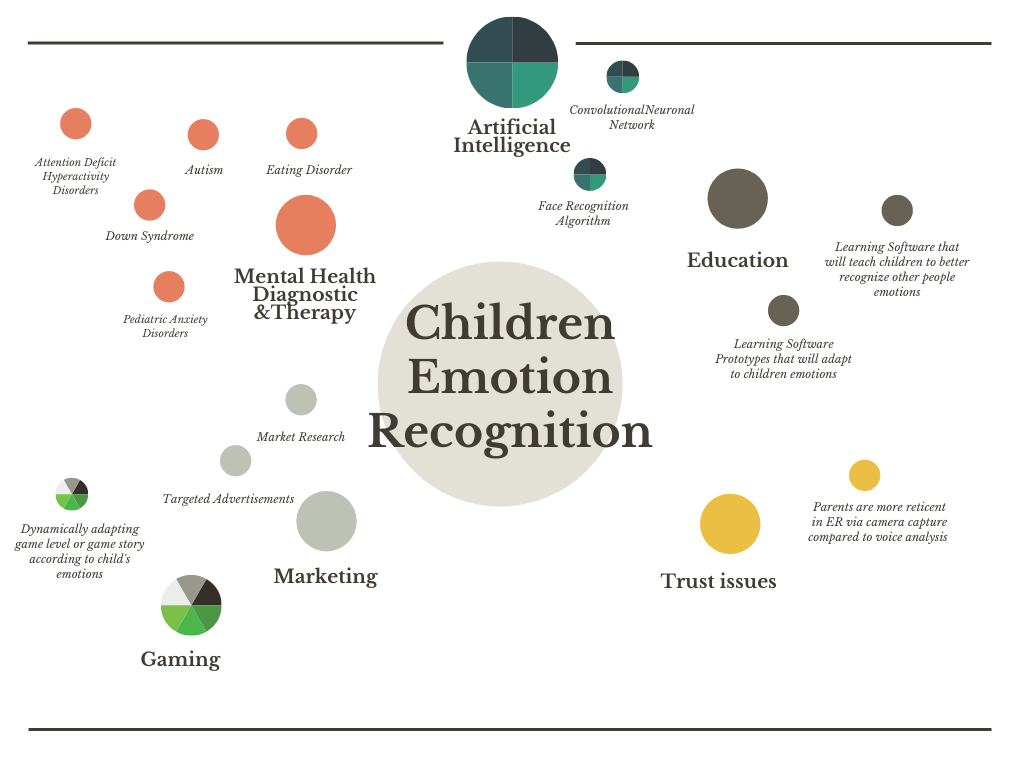
\includegraphics[scale=0.6]{MindMap.png}
  \caption{Children Emotion Recognition Usages and Potential Problems}
\end{figure}
  

\subsection{How?}
\label{subsection:how}
\paragraph{}
We designed a convolutional neural network which was used to process the images and clasify kids emotions, offering a distribution of each emotion.

\section{Paper structure and original contributions(s)}
\label{section:structure}
\paragraph{}
The main contribution of this report is to present an intelligent algorithm for solving the problem of facial emotion recognition for children.

\paragraph{}
The second contribution of this report consists of building an intuitive, easy-to-use and user friendly software application. Our aim is to build an algorithm that will help adult specialists working in social services to better recognize children emotions even when they are not able to verbalize or write down their potential traumatic experiences.

\paragraph{}
The third contribution of this thesis consists of providing a comparison between the accuracy results obtained while using FER algorithm and our final solution.

\paragraph{}
The present work contains \cite{LoBlue2015}, \cite{Camras1996}, \cite{Kasari2001}, \cite{Bal2010}, \cite{Revina2018} bibliographical references and is structured in five chapters as follows.

\paragraph{}
The first chapter (this one) is a short introduction about the paper and the motivation behind it, describing the facial emotion recognition evolution and why it is important to apply these features also on infant facial expressions.

\paragraph{}
The second chapter describes will focus on the scientific problem that our application is trying to solve.

\paragraph{}
The third chapter focuses on the state of art and the proposed approach.

\paragraph{}
The fourth chapter will present a comparison between our chosen approach, data and results when trying to solve the above mentioned problem and another the results of another existing approach.

\paragraph{}
The fifth chapter will present our conclusions and our future work related to this application.

\chapter{Scientific Problem}
\label{section:scientificProblem}

\section{Problem definition}
\label{section:problemDefinition}
\paragraph{}
The problem we want to solve is kids emotion recognition meaning identifying children emotions during their activities.

\paragraph{}
We have identified two main uses of our application:
\begin{enumerate}
  \item Kindergarten teachers could use such a tool to independently identify children emotions while they are playing or are performing some educative task at a computer in order to assess their competencies level and provide them more targeted content, suitable for their needs.
  \item Social assistants often need to take care and provide physical and emotional comfort to children who were abused at an earlier stage in their lifetime. If the infant has not yet developed his vocabulary or he was not sufficiently stimulated in his first years of life, he might be unable to talk about his experiences, nor about his emotions in relation with those experiences.
\end{enumerate}

\paragraph{}
In this context, a solution that uses an intelligent algorithm to correctly identify children emotions could be extremely helpful in order to provide specific care and treatment in accord with their specific need.

\paragraph{}
Advantages of solving the problem using an intelligent algorithm:
\begin{itemize}
	\item it could accurately spot the emotions much faster than trying to guess infants' emotions without using any other tool
 	\item the result of the analysis would be independent from social assistant's level of empathy when determining the children emotions
 	\item in some cases, it could be nearly impossible for a human being to correctly identify all the micro-expressions hidden in an youngster mimic
\end{itemize}

\paragraph{}
Disadvantages of solving the problem using an intelligent algorithm:
\begin{itemize}
	\item it may require a lot of training an re-training in order to reach an optimized model suited to accurately determine children emotions
 	\item even the best found solution cannot be 100\% accurate in providing a result
\end{itemize}

\chapter{State of art/Related work}
\label{chapter:stateOfArt}
\section{State of art}
\paragraph{}
Some of the most relevant methods used until now in attempt to solve the facial emotion recognition problem obtained the following results:
\begin{enumerate}
  \item In their research paper \cite{Cai2018}, the experimental results on four benchmark expression databases have demonstrated that the CNN with the proposed island loss (IL-CNN) outperforms the baseline CNN models with either traditional softmax loss or center loss and achieves comparable or better performance compared with the state-of-the-art methods for facial expression recognition.
  
  DataSet used: CK+
  Results: 90.66\%
  \item Another approach \cite{Hinton2006} states that high-dimensional data can be converted to low-dimensional codes by training a multilayer neural network with a small central layer to reconstruct high-dimensional input vectors. Gradient descent can be used for fine-tuning the weights in such "autoencoder" networks, which could perform well only if the initial weights are close to a good solution. The solution is initializing the weights that allows deep autoencoder networks to learn low-dimensional codes that work much better than principal components analysis as a tool to reduce the dimensionality of data.
  
  Dataset used: JAFFE
  Results: 95.79\%
\end{enumerate}
\paragraph{}
Although they achieved spectacular results, none of them were using a database that contained only children images. This is the gap that we are trying to fill in with the results of our application.

\section{Tools}
\paragraph{}
In order to build our intelligent application, we have used the following libraries and tools:
\begin{itemize}
  \item TensorFlow: is a Python library for fast numerical computing created and released by Google. It is a foundation library that can be used to create Deep Learning models directly or by using wrapper libraries that simplify the process built on top of TensorFlow. \cite{tensorflow}
  \item Keras: is an open-source neural-network library written in Python. It is capable of running on top of TensorFlow, Microsoft Cognitive Toolkit, R, Theano, or PlaidML. Designed to enable fast experimentation with deep neural networks, it focuses on being user-friendly, modular, and extensible.\cite{keras}
\end{itemize}














\chapter{Proposed approach}
\label{chapter:proposedApproach}

\section{Application}
\label{section:application}

\textbf{Neural Networks} are a set of algorithms, modeled mainly after the human brain, that are designed to identify and recognize different types of patterns. The patterns that the algorithms recognize are numerical, contained in vectors, into which all real-world data, be it images, sound, text or time series, must be translated.
Neural networks can be seen as a clustering and classification layer on top of the data that needs to be stored and managed. They help to group unlabeled data according to similarities between the example inputs.
All classification tasks depend upon labeled datasets. In other words, humans must transfer their existing knowledge to the dataset so a neural network to learn the correlation between labels and data. This is known as supervised learning and brings value for:
\begin{itemize}
	\item Detect faces, identify people in images, \textbf{recognize facial expressions}
	\item Recognize gestures in video
	\item Identify objects in images
\end{itemize} and many others.\cite{skymindneural}

\paragraph{}
A \textbf{Convolutional Neural Network (CNN)} is a type of artificial neural network used in image recognition and processing that is specifically designed to process data based on its pixels. A CNN is a Deep Learning algorithm which can take in an input image, assign importance (weights) to various aspects in the image and be able to differentiate one from the other. Traditional neural networks are not ideal for image processing and must be fed images in reduced-resolution pieces. CNN have their "neurons" (nodes) arranged more like those of the frontal lobe, the area responsible for processing visual stimuli in humans.\cite{searchwhat}

\begin{center}
    \captionof{table}{Arhitecture of our CNN}
    \begin{longtable}{|| c c c ||} 
    \hline Model: "sequential" & & \\
    \hline
    Layer (type) & Output Shape & Param \#  \\ [2ex] 
    \hline\hline
    conv2d (Conv2D) & (None, 46, 46, 64) & 640  \\ 
    \hline
    conv2d\_1 (Conv2D) & (None, 46, 46, 64) & 36928  \\
    \hline
    batch\_normalization (BatchNo) & (None, 46, 46, 64) & 256  \\
    \hline
    max\_pooling2d (MaxPooling2D) & (None, 23, 23, 64) & 0  \\
    \hline
    dropout (Dropout) & (None, 23, 23, 64) & 0  \\
    \hline
    conv2d\_2 (Conv2D) & (None, 23, 23, 128) & 73856  \\
    \hline
    batch\_normalization\_1 (Batch) & (None, 23, 23, 128) & 512  \\
    \hline
    conv2d\_3 (Conv2D) & (None, 23, 23, 128) & 147584  \\
    \hline
    batch\_normalization\_2 (Batch) & (None, 23, 23, 128) & 512  \\
    \hline
    max\_pooling2d\_1 (MaxPooling2D) & (None, 11, 11, 128) & 0  \\
    \hline
    dropout\_1 (Dropout) & (None, 11, 11, 128) & 0  \\
    \hline
    conv2d\_4 (Conv2D) & (None, 11, 11, 256) & 295168  \\
    \hline
    batch\_normalization\_3 (Batch) & (None, 11, 11, 256) & 1024\\
    \hline
    conv2d\_5 (Conv2D) & (None, 11, 11, 256) & 590080 \\
    \hline
    batch\_normalization\_4 (Batch) & (None, 11, 11, 256) & 1024\\
    \hline
    max\_pooling2d\_2 (MaxPooling2D) & (None, 5, 5, 256) & 0\\
    \hline
    dropout\_2 (Dropout) & (None, 5, 5, 256) & 0\\
    \hline
    conv2d\_6 (Conv2D) & (None, 5, 5, 512) & 1180160\\
    \hline
    batch\_normalization\_5 (Batch) & (None, 5, 5, 512) & 2048\\
    \hline
    conv2d\_7 (Conv2D) & (None, 5, 5, 512) & 2359808\\
    \hline
    batch\_normalization\_6 (Batch) & (None, 5, 5, 512) & 2048\\
    \hline
    max\_pooling2d\_3 (MaxPooling2D) & (None, 2,2, 512) & 0\\
    \hline
    dropout\_3 (Dropout) & (None, 2, 2, 512) & 0\\
    \hline
    flatten (Flatten) & (None, 2048) & 0\\
    \hline
    dense (Dense) & (None, 512) & 1049088\\
    \hline
    dropout\_4 (Dropout) & (None, 512) & 0\\
    \hline
    dense\_1 (Dropout) & (None, 256) & 131328\\
    \hline
    dropout\_5 (Dropout) & (None, 256) & 0\\
    \hline
    dense\_2 (Dense) & (None, 128) & 32896\\
    \hline
    dropout\_6 (Dropout) & (None, 128) & 0\\
    \hline
    dense\_3 (Dense) & (None, 7) & 903 \\
    \hline
    Total params: 5,905,863 & &\\
    Trainable params: 5,902,151 & &\\
    Non-trainable params: 3,712 & & \\
    \hline
  \end{longtable}
\end{center}

\paragraph{}
Our application offers more functionalities:
\begin{itemize}
  \item Choosing input type between image and video
  \item Choosing model to use for prediction between CAFFE and FER
  \item Image/Video loading mechanism
  \item Results visualizing, including some charts for video input (emotion distribution \& emotion transition during the video)
\end{itemize}


\begin{figure}[!ht]
  \label{fig::app1}
  \centering
  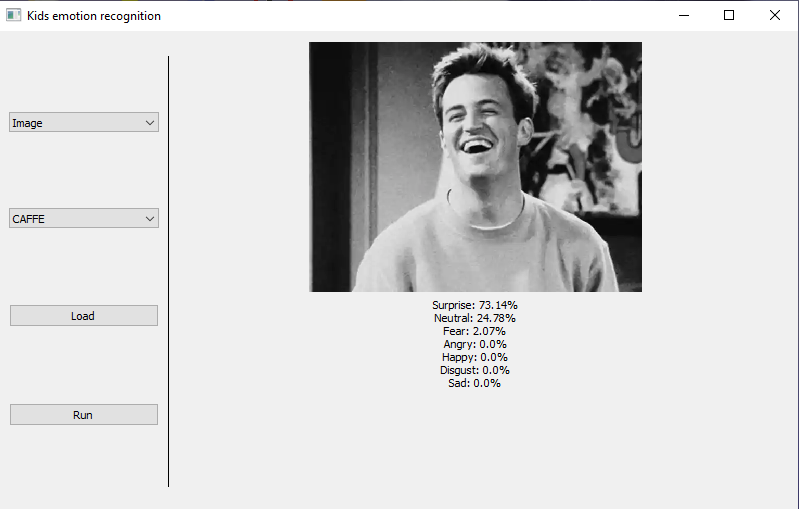
\includegraphics[width=0.85\textwidth]{Images/app_1.png}
  \caption{Image classification with our app}
\end{figure}


\begin{figure}[!ht]
  \label{fig::app2}
  \centering
  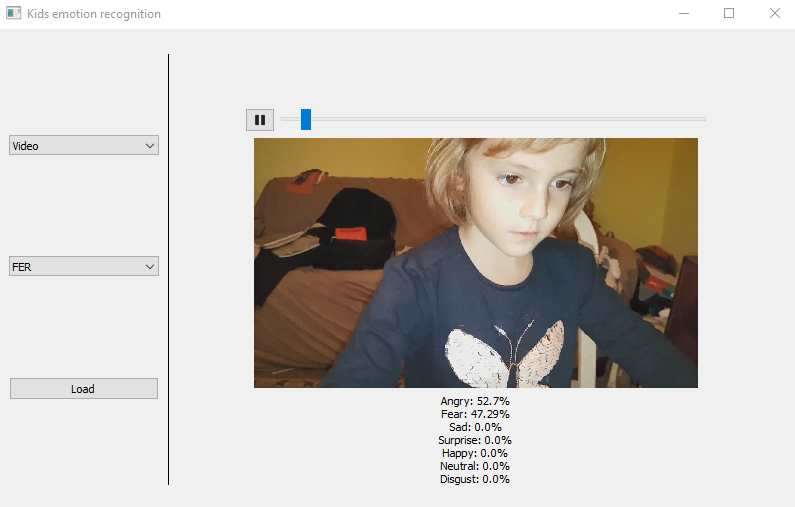
\includegraphics[width=0.85\textwidth]{Images/app_2.png}
  \caption{Video classification with our app}
\end{figure}


\begin{figure}[!ht]
  \label{fig::app3}
  \centering
  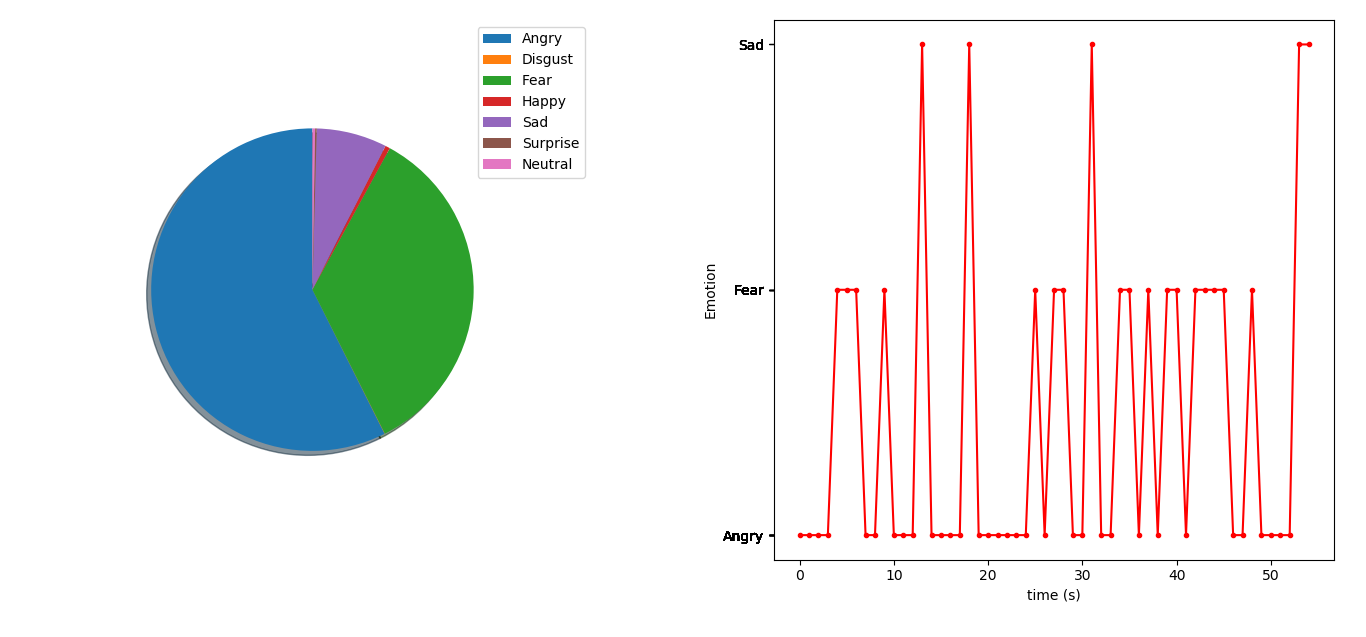
\includegraphics[width=0.85\textwidth]{Images/app_3.png}
  \caption{Charts for video: emotion distribution and emotion transition}
\end{figure}

\newpage

\section{Methodology}
\label{section:methodology}

\paragraph{}
Our main purpose was to use an existing algorithm proven to be efficient at identifying adult's facial emotions, train it using CAFE \cite{LoBlue2015} data set and finally to integrate it in our user-friendly application capable of providing instant statistical feedback regarding the child emotion.

\begin{figure}[!ht]
  \label{fig::architecture}
  \centering
  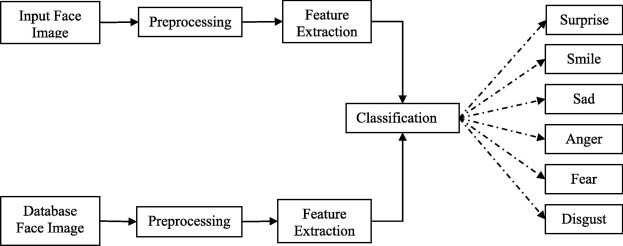
\includegraphics[width=0.85\textwidth]{Images/arhitecture.jpg}
  \caption{Architecture of face expression recognition system \cite{Revina2018}}
\end{figure}

\begin{itemize}
	\item What are criteria you are using to evaluate your method?
  \paragraph{}
  In order to evaluate our method we took into consideration two aspects: correctness of results and usability.
  Results' correctness can be best measured by analyzing the accuracy of our model in comparison with accuracy obtained by the existing algorithm model.
  \paragraph{}
  The accuracy of a model is usually determined after the model parameters are learned and fixed and no learning is taking place.
  \paragraph{}
  The usability aspect has been measured by the easiness with which an user could obtain the required result. In our case, the user only needs to press on the button to upload a photo, select a photo and check the result of the emotions displayed.
	\item What specific hypotheses does your experiment test? Describe the experimental methodology that you used.
  \paragraph{}
  We have initially trained our algorithm by providing CAFE data set as input but we have realised that some of the labels where wrongly attributed (ex. sad emotion looked very similar to neutral emotion).
  \paragraph{}
  Another enhancement brought to the data set was to remove the images that were containing open mouth images and where the emotion was difficult to detect.
	\item What are the dependent and independent variables?
  \begin{itemize}
    \item Learning Rate: 0.001
    \item Adam Optimizer
    \item Categorical Cross-Entropy Loss
  \end{itemize}

	\item What is the training/test data that was used, and why is it realistic or interesting? Exactly what performance data did you collect and how are you presenting and analyzing it? Comparisons to competing methods that address the same problem are particularly useful.
  \paragraph{FER 2013 Dataset}
  \begin{itemize}
    \item Does not contain children images
    \item Traning accuracy (90\% from dataset): 98.64\% - Test accuracy (10\% from dataset): 67.24\% (a bit of overfitting)
  \end{itemize}

  \paragraph{CAFFE Dataset}

  \begin{itemize}
    \item Data are unbalanced
    \item Labeling seems to be wrong (sad seems neutral or others)
    \item Has open mouth faces (e.g. for sad, neutral)
    \item Traning accuracy (90\% from dataset): 89.94\% - Test accuracy (10\% from dataset): 67.59\% (a bit of overfitting) - also removing the open mouth images
    \item Contains only children images
  \end{itemize}

 \paragraph{Videos}
   \begin{itemize}
    \item Not all the frames from the video were relevant for the data set
  \end{itemize}

\end{itemize}

\section{Data}
\label{section:data}

\paragraph{FER}
The data consists of 48x48 pixel grayscale images of faces. The faces have been automatically registered so that the face is more or less centered and occupies about the same amount of space in each image. The task is to categorize each face based on the emotion shown in the facial expression in to one of seven categories (0=Angry, 1=Disgust, 2=Fear, 3=Happy, 4=Sad, 5=Surprise, 6=Neutral).

\paragraph{}
train.csv contains two columns, "emotion" and "pixels". The "emotion" column contains a numeric code ranging from 0 to 6, inclusive, for the emotion that is present in the image. The "pixels" column contains a string surrounded in quotes for each image. The contents of this string a space-separated pixel values in row major order. test.csv contains only the "pixels" column and your task is to predict the emotion column.

\paragraph{CAFFE}
To train the algorithm for facial recognition we have used the data set provided by the Child Study Center at Rutgers University, New Jersey.
The Child Affective Facial Expressions Set (CAFE)\cite{LoBlue2015} represents the first large representative database of children posing using many facial expressions.
% \begin{figure}[htbp]
% 	\centerline{\includegraphics{child emotions.png}}
% 	\caption{Example of the child images included in the CAFE data set.}
% 	\label{swarmsize}
% \end{figure}
\paragraph{}
This data set consists of approximately 1200 photographs of over 100 children racially and ethnically diverse (90 female models and 64 male models: 27 African American, 16 Asian, 77 Caucasian/European American, 23 Latino, and 11 South Asian)with ages between 2 and 8 years old, that are posing 7 different facial expressions:  happy, angry, sad, fearful, surprise, neutral and disgust.

\paragraph{}
The institute focuses their research on the cognitive, emotional and perceptual development of infants and children. To gather all these visual records, the institute is inviting all families having a child with age between 3 and 8 years, to take part in the study by bringing their child to a session of 30-45 minutes of computer interactive games or of a stimulating reading session. The children are verbally invited to pose each of the emotion with their mouth open and with their mouth closed.

\paragraph{Videos}
To gather additional data for training, we also took into consideration fragmenting videos that contained children as main characters and capture the frames which contained a dominant emotion and add it to our data set. This step has improved the accuracy of our algorithm and we made sure that the label reflected correctly the children emotions.

\section{Results}
\label{section:results}

% \begin{figure}[htbp]
% 	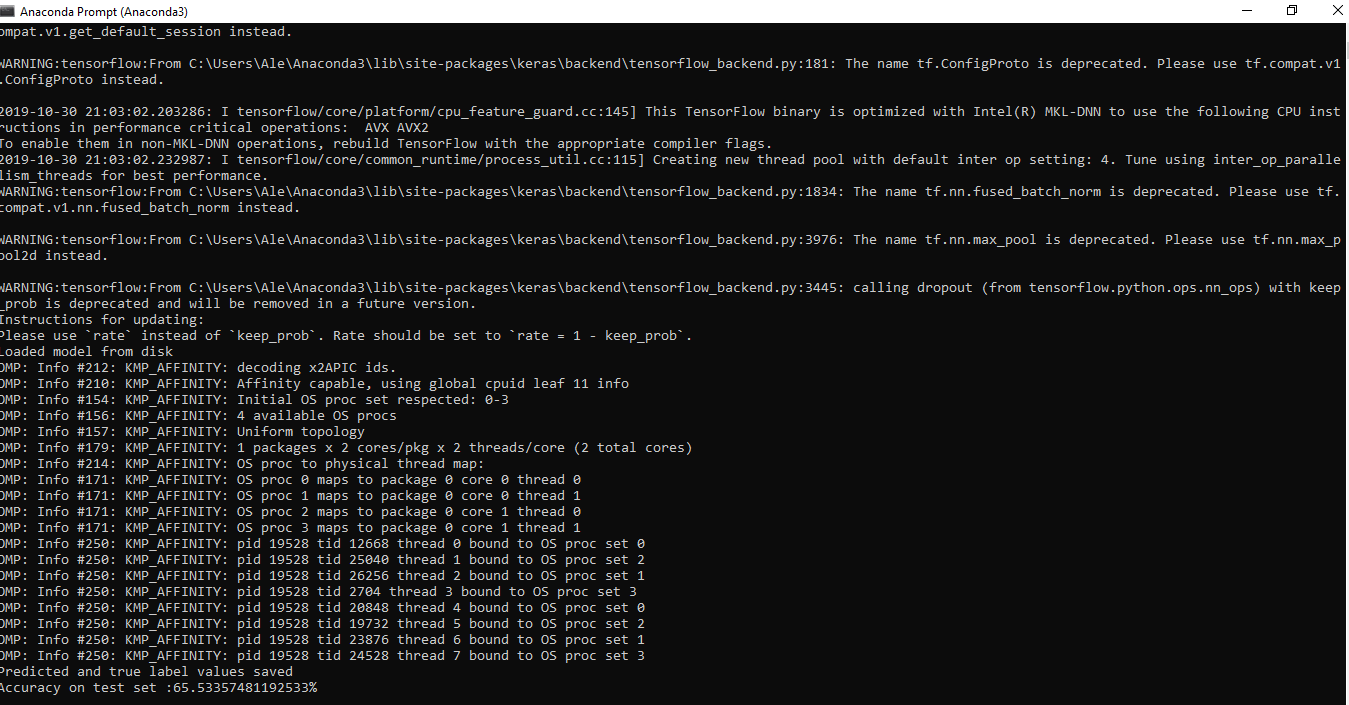
\includegraphics{accuracy-test-program.png}
% 	\caption{Accuracy Results}
% 	\label{swarmsize}
% \end{figure}

\begin{itemize}
  \item FER: Traning acc (90\% from dataset): 98.64\% - Test acc (10\% from dataset): 71.161\% (a bit of overfitting)
  \item CAFFE: Traning acc (90\% from dataset): 89.94\% - Test acc (10\% from dataset): 65.5335\% (a bit of overfitting) - also removing the open mouth images
  \item Videos: Traning acc (90\% from dataset): 89.94\% - Test acc (10\% from dataset): 65.5335\% (a bit of overfitting)
\end{itemize}

\section{Discussion}
\label{section:discussion}

\begin{itemize}
	\item Is your hypothesis supported?
  \paragraph{}
  Lots of improvements can be made to our algorithm in order to increase its accuracy, but given the fact that our data set was unbalanced and we were still able to achieve a better result than FER-2013 gives us the confidence that if we continue to broaden our database, we will obtain even better results.
	\item What conclusions do the results support about the strengths and weaknesses of your method compared to other methods?
  \paragraph{}
  A larger balanced data set with child faces is needed to obtain better results. Even so, the children facial emotion recognition is at its early stages of development and once a more consistent database will be created, our application results will increase as preponderantly.
	\item How can the results be explained in terms of the underlying properties of the algorithm and/or the data.
  \paragraph{}
  Overfitting could happen sometimes (depends on the dataset), but the algorithm is pretty accurate as a human can be.
\end{itemize}

\chapter{Conclusion and future work}
\label{chapter:concl}
\paragraph{}
Although we were able to build an easy-to-use application, capable to reflect the emotion of the child captured in an image sample, further improvements can be made to our model, to increase its accuracy and overall results. The development of this application made us more aware of the challenges faced when training an intelligent algorithm and trying to find an optimized solution without harming any other aspect.

\paragraph{}
Since the data sets that contains children facial images are not large enough and are not evenly distributed the results cannot be as accurate as desired. However, future steps can be taken in order to artificially expand our database by increasing their number and variety. For \textbf{data augmentation} we could use techniques such as: Image Flip, Pepper Noise, Additive Gaussian Noise etc. These filters although they would be applied on the same images that are already existing in our database, would be able to increase the accuracy and variety of our images.


\bibliographystyle{plain}
%\bibliography{BibAll}
\begin{thebibliography}{1}
  \bibitem{stanford} http://deeplearning.stanford.edu/tutorial/supervised/ConvolutionalNeuralNetwork/

  \bibitem{machinelearning} https://machinelearningmastery.com/convolutional-layers-for-deep-learning-neural-networks/

  \bibitem{searchwhat} https://searchenterpriseai.techtarget.com/definition/convolutional-neural-network

  \bibitem{skymind} https://skymind.ai/wiki/convolutional-network

  \bibitem{skymindneural} https://skymind.ai/wiki/neural-network

  \bibitem{towards} https://towardsdatascience.com/a-comprehensive-guide-to-convolutional-neural-networks-the-eli5-way-3bd2b1164a53

  \bibitem{tensorflow} https://machinelearningmastery.com/introduction-python-deep-learning-library-tensorflow/

   \bibitem{keras}
   https://en.wikipedia.org/wiki/Keras

    \bibitem{fer2013}
    https://github.com/gitshanks/fer2013/blob/master/README.md


\bibitem{LoBlue2015}
Vanessa LoBue and Cat Thrasher
\textit{The Child Affective Facial Expression (CAFE) set: validity and reliability from untrained adults}.
Frontiers in Emotion Science, Psychology, 2015.
\\\texttt{https://doi.org/10.3389/fpsyg.2014.01532}


\bibitem{Camras1996}
Camras, L. A., Sachs-Alter, E., and Ribordy, S. C. (1996). \textit{Emotion understanding in maltreated children: Recognition of facial expressions and integration with other emotion cues.}
Emotional development in atypical children (p.203-225) Lawrence Erlbaum Associates, Inc, 1996
\\\texttt{https://psycnet.apa.org/record/1996-98206-011}


\bibitem{Kasari2001}
Connie Kasari, Stephanny F. N. Freeman, and Margaret A. Hughes
\textit{Emotion Recognition by Children With Down Syndrome.}.
American Journal on Mental Retardation: January 2001, Vol. 106, No. 1, pp. 59-72.
\\\texttt{https://doi.org/10.1352/0895-8017}

\bibitem{Bal2010}
Elgiz Bal, Emily Harden, Damon Lamb, Amy Vaughan Van Hecke, John W. Denver, Stephen W. Porges
\textit{Emotion Recognition in Children with Autism Spectrum Disorders: Relations to Eye Gaze and Autonomic State}.
Journal of Autism and Developmental Disorders
March 2010, Volume 40, Issue 3, pp 358-370
\\\texttt{https://doi.org/10.1007/s10803-009-0884-3}

\bibitem{Revina2018}
I.Michael Revina, W.R. Sam Emmanuel
\textit{A Survey on Human Face Expression Recognition Techniques}.
Journal of King Saud University - Computer and Information Sciences
September 2018, pp 2
\\\texttt{https://doi.org/10.1016/j.jksuci.2018.09.002}

\bibitem{Cai2018}
Jie Cai, Zibo Meng, Ahmed Shehab Khan, Zhiyuan Li, James O'Reilly, Yan Tong
\textit{Island Loss for Learning Discriminative Features in Facial Expression Recognition}.
 2018 13th IEEE International Conference on Automatic Face and Gesture Recognition (FG 2018)
May 2018, pp 2
\\\texttt{https://doi.org/10.1109/FG.2018.00051}

\bibitem{Hinton2006}
G.E. Hinton, R.R. Salakhutdinov
\textit{Reducing the Dimensionality of Data with Neural Networks}.
Science 313(5786):504-7
August 2006
\\\texttt{https://doi.org/10.1126/science.1127647}

\end{thebibliography}
\end{document}

